\documentclass[english,man]{apa6}

\usepackage{amssymb,amsmath}
\usepackage{ifxetex,ifluatex}
\usepackage{fixltx2e} % provides \textsubscript
\ifnum 0\ifxetex 1\fi\ifluatex 1\fi=0 % if pdftex
  \usepackage[T1]{fontenc}
  \usepackage[utf8]{inputenc}
\else % if luatex or xelatex
  \ifxetex
    \usepackage{mathspec}
    \usepackage{xltxtra,xunicode}
  \else
    \usepackage{fontspec}
  \fi
  \defaultfontfeatures{Mapping=tex-text,Scale=MatchLowercase}
  \newcommand{\euro}{€}
\fi
% use upquote if available, for straight quotes in verbatim environments
\IfFileExists{upquote.sty}{\usepackage{upquote}}{}
% use microtype if available
\IfFileExists{microtype.sty}{\usepackage{microtype}}{}

% Table formatting
\usepackage{longtable, booktabs}
\usepackage{lscape}
% \usepackage[counterclockwise]{rotating}   % Landscape page setup for large tables
\usepackage{multirow}		% Table styling
\usepackage{tabularx}		% Control Column width
\usepackage[flushleft]{threeparttable}	% Allows for three part tables with a specified notes section
\usepackage{threeparttablex}            % Lets threeparttable work with longtable

% Create new environments so endfloat can handle them
% \newenvironment{ltable}
%   {\begin{landscape}\begin{center}\begin{threeparttable}}
%   {\end{threeparttable}\end{center}\end{landscape}}

\newenvironment{lltable}
  {\begin{landscape}\begin{center}\begin{ThreePartTable}}
  {\end{ThreePartTable}\end{center}\end{landscape}}

  \usepackage{ifthen} % Only add declarations when endfloat package is loaded
  \ifthenelse{\equal{\string man}{\string man}}{%
   \DeclareDelayedFloatFlavor{ThreePartTable}{table} % Make endfloat play with longtable
   % \DeclareDelayedFloatFlavor{ltable}{table} % Make endfloat play with lscape
   \DeclareDelayedFloatFlavor{lltable}{table} % Make endfloat play with lscape & longtable
  }{}%



% The following enables adjusting longtable caption width to table width
% Solution found at http://golatex.de/longtable-mit-caption-so-breit-wie-die-tabelle-t15767.html
\makeatletter
\newcommand\LastLTentrywidth{1em}
\newlength\longtablewidth
\setlength{\longtablewidth}{1in}
\newcommand\getlongtablewidth{%
 \begingroup
  \ifcsname LT@\roman{LT@tables}\endcsname
  \global\longtablewidth=0pt
  \renewcommand\LT@entry[2]{\global\advance\longtablewidth by ##2\relax\gdef\LastLTentrywidth{##2}}%
  \@nameuse{LT@\roman{LT@tables}}%
  \fi
\endgroup}


\ifxetex
  \usepackage[setpagesize=false, % page size defined by xetex
              unicode=false, % unicode breaks when used with xetex
              xetex]{hyperref}
\else
  \usepackage[unicode=true]{hyperref}
\fi
\hypersetup{breaklinks=true,
            pdfauthor={},
            pdftitle={Consistency and variability in word learning across languages},
            colorlinks=true,
            citecolor=blue,
            urlcolor=blue,
            linkcolor=black,
            pdfborder={0 0 0}}
\urlstyle{same}  % don't use monospace font for urls

\setlength{\parindent}{0pt}
%\setlength{\parskip}{0pt plus 0pt minus 0pt}

\setlength{\emergencystretch}{3em}  % prevent overfull lines

\ifxetex
  \usepackage{polyglossia}
  \setmainlanguage{}
\else
  \usepackage[english]{babel}
\fi

% Manuscript styling
\captionsetup{font=singlespacing,justification=justified}
\usepackage{csquotes}
\usepackage{upgreek}

 % Line numbering
  \usepackage{lineno}
  \linenumbers


\usepackage{tikz} % Variable definition to generate author note

% fix for \tightlist problem in pandoc 1.14
\providecommand{\tightlist}{%
  \setlength{\itemsep}{0pt}\setlength{\parskip}{0pt}}

% Essential manuscript parts
  \title{Consistency and variability in word learning across languages}

  \shorttitle{Consistency and variability in word learning}


  \author{Mika Braginsky\textsuperscript{1}, Daniel Yurovsky\textsuperscript{2}, Virginia A. Marchman\textsuperscript{3}, \& Michael C. Frank\textsuperscript{3}}

  \def\affdep{{"", "", "", ""}}%
  \def\affcity{{"", "", "", ""}}%

  \affiliation{
    \vspace{0.5cm}
          \textsuperscript{1} Department of Brain and Cognitive Sciences, Massachusetts Institute of
Technology\\
          \textsuperscript{2} Department of Psychology, University of Chicago\\
          \textsuperscript{3} Department of Psychology, Stanford University  }

 % If no author_note is defined give only author information if available
      \newcounter{author}
                              \authornote{
            Correspondence concerning this article should be addressed to Mika Braginsky. E-mail: \href{mailto:mikabr@mit.edu}{\nolinkurl{mikabr@mit.edu}}
          }
                                                              

  \abstract{Why do children learn some words earlier than others? The order in which
words are acquired can provide clues about the mechanisms of word
learning. In a large-scale corpus analysis, we use data from over 38,000
children to estimate the acquisition trajectories of around 400 words in
ten languages, predicting them on the basis of independently-derived
environmental and conceptual factors. We examine the consistency and
variability of these predictors across languages, by lexical category,
and over development. The ordering of predictors across languages is
quite similar, suggesting similar processes in operation. In contrast,
the ordering of predictors across different lexical categories is
distinct, in line with theories that posit distinct factors at play in
the acquisition of content words and function words. By leveraging data
at a significantly larger scale than previous work, our analyses
identify candidate generalizations about the processes underlying word
learning across languages.}
  \keywords{word learning, language acquisition, corpus analysis \\

    
  }





\usepackage{amsthm}
\newtheorem{theorem}{Theorem}
\newtheorem{lemma}{Lemma}
\theoremstyle{definition}
\newtheorem{definition}{Definition}
\newtheorem{corollary}{Corollary}
\newtheorem{proposition}{Proposition}
\theoremstyle{definition}
\newtheorem{example}{Example}
\theoremstyle{definition}
\newtheorem{exercise}{Exercise}
\theoremstyle{remark}
\newtheorem*{remark}{Remark}
\newtheorem*{solution}{Solution}
\begin{document}

\maketitle

\setcounter{secnumdepth}{0}



In spite of tremendous individual variation in rate of development (1),
the first words that children utter are strikingly consistent (2, 3):
they tend to talk about important people in their life (\enquote{mom},
\enquote{dad}), social routines (\enquote{hi}, \enquote{uh oh}), animals
(\enquote{dog}, \enquote{duck}), and foods (\enquote{milk},
\enquote{banana}). As children learn from their experiences and
according to their own interests ({\textbf{???}}, 4), their vocabulary
grows rapidly, typically adding more nouns, but also verbs
(\enquote{go}) and other predicates (\enquote{hot}) to their production
repertoires. Over just their first three years, children learn hundreds
or even thousands of words (5, 6). Why are some words learned so early
and some much later?

This simple question about the order of the acquisition of first words
can provide a window into the nature of children's language learning.
Posed as a statistical problem, the challenge is to find what variables
best predict the age at which different words are acquired. Previous
work using this approach has revealed that in English, within a lexical
category (e.g., nouns, verbs), words that are more frequent in speech to
children are likely to be learned earlier (7). And further studies have
found evidence that a variety of other semantic and linguistic factors
are related to word acquisition (8--12).

But these exciting findings are limited in their generality because they
use different datasets, focus on different predictors, and almost
exclusively analyze English data. They do not allow for cross-linguistic
comparison of the relative importance of the many relevant factors under
consideration in children from different language communities. Such
cross-linguistic comparisons are critical, as identifying commonalities
(and differences) across languages is our best strategy for uncovering
the universal mechanisms that are in play for all children and
differentiating them from patterns of acquisition that emerge due to the
particulars of a given language or culture (13, 14). Our goal is to
extend these classic approaches by assessing the degree to which the
predictors of word learning are consistent across different languages
and cultures, as well as whether there are similar patterns across
different word types (e.g., nouns vs.~verbs).

To conduct cross-linguistic comparisons, we rely on data from Wordbank
(\href{http://wordbank.stanford.edu}{wordbank.stanford.edu}) (15).
Wordbank is an open repository of cross-linguistic language development
data that aggregates administrations of the MacArthur-Bates
Communicative Development Inventory (1), a family of parent-report
vocabulary checklists, and currently includes data from more than 60,000
children. By aggregating across large samples, idiosyncratic patterns of
individual variation are less likely to overpower general trends in
which words are relatively easy or hard to learn, allowing us to
investigate what features affect their acquisition across languages.

In our analyses, we integrate estimates of words' acquisition
trajectories from Wordbank with characterizations of the word learning
environment from the CHILDES database (16) and elsewhere, a
data-integration methodology originated by (7). Using this approach, we
examine the impact of multiple environmental and conceptual factors. To
measure environmental input, we estimated each word's frequency, mean
length of utterance (MLU), frequency as sole utterance constituent, and
frequency in utterance-final position. To measure conceptual factors, we
obtained ratings of each word's concreteness, valence, arousal, and
association with babies from previously collected norms. We used these
measures to predict words' acquisition trajectories, assessing the
relative contributions of each, as well as how they change over
development and interact with lexical category. These analyses address
two important questions.

First, we ask about the degree of consistency across languages in the
relative importance of predictors. Consistency in the ordering of
predictors would suggest that similar information sources are important
for learners, regardless of language. Such evidence would point to the
importance of similar learning mechanisms across languages despite
superficial dissimilarities (e.g., greater morphological complexity in
Russian and Turkish, greater phonological complexity in Danish).
Conversely, variability would reveal the degree to which learners face
different challenges in learning different languages.

Second, we ask which lexical categories are most influenced by
environmental factors, like frequency and utterance length, compared
with conceptual factors like concreteness and valence. Division of
dominance theory suggests that nouns might be more sensitive to
conceptual factors, while predicates and closed-class words might be
more sensitive to environmental (linguistic) factors (17). And on
syntactic bootstrapping theories (18), nouns are argued to be learned
via frequent co-occurrence (operationalized by frequency) while verbs
might be more sensitive to syntactic factors (operationalized here by
utterance length) (19). Thus, examining the relative contribution of
different predictors across lexical categories can help test the
predictions of influential theories of acquisition.

\section*{Approach}\label{approach}
\addcontentsline{toc}{section}{Approach}

\begin{table}[b]
\centering
\begin{tabular}{lrrr}
  \hline
Language & CDI Items & N production & N comprehension \\ 
  \hline
Croatian & 390 & 627 & 250 \\ 
  Danish & 383 & 6,112 & 2,398 \\ 
  English & 393 & 5,967 & 1,821 \\ 
  French & 396 & 1,364 & 537 \\ 
  Italian & 396 & 1,400 & 648 \\ 
  Norwegian & 381 & 7,466 & 2,374 \\ 
  Russian & 410 & 1,805 & 768 \\ 
  Spanish & 399 & 1,872 & 778 \\ 
  Swedish & 371 & 1,367 & 467 \\ 
  Turkish & 396 & 3,537 & 1,115 \\ 
   \hline
\end{tabular}
\caption{Dataset statistics for acquisition data from Wordbank.} 
\label{table:lang_stats}
\end{table}

To estimate the trajectory of words' acquisition, we used vocabulary
data collected using CDI instruments adapted in many different
languages, including both Words \& Gestures (WG) forms for younger
children and Words \& Sentences (WS) forms for older children. When
filling out a CDI form, parents are either asked to indicate whether
their child \enquote{understands} (comprehension) or
\enquote{understands and says} (production) each of around 400-700
words. Typically, both comprehension and production are queried for
younger children and only production is queried for older children, but
details vary from adaptation to adaptation. We use data from the items
on the WG form for our comprehension measure, and data from the items in
common between the WG and WS forms for our production measure. Table 1
gives an overview of our acquisition data (20--31).

\begin{figure*}

{\centering 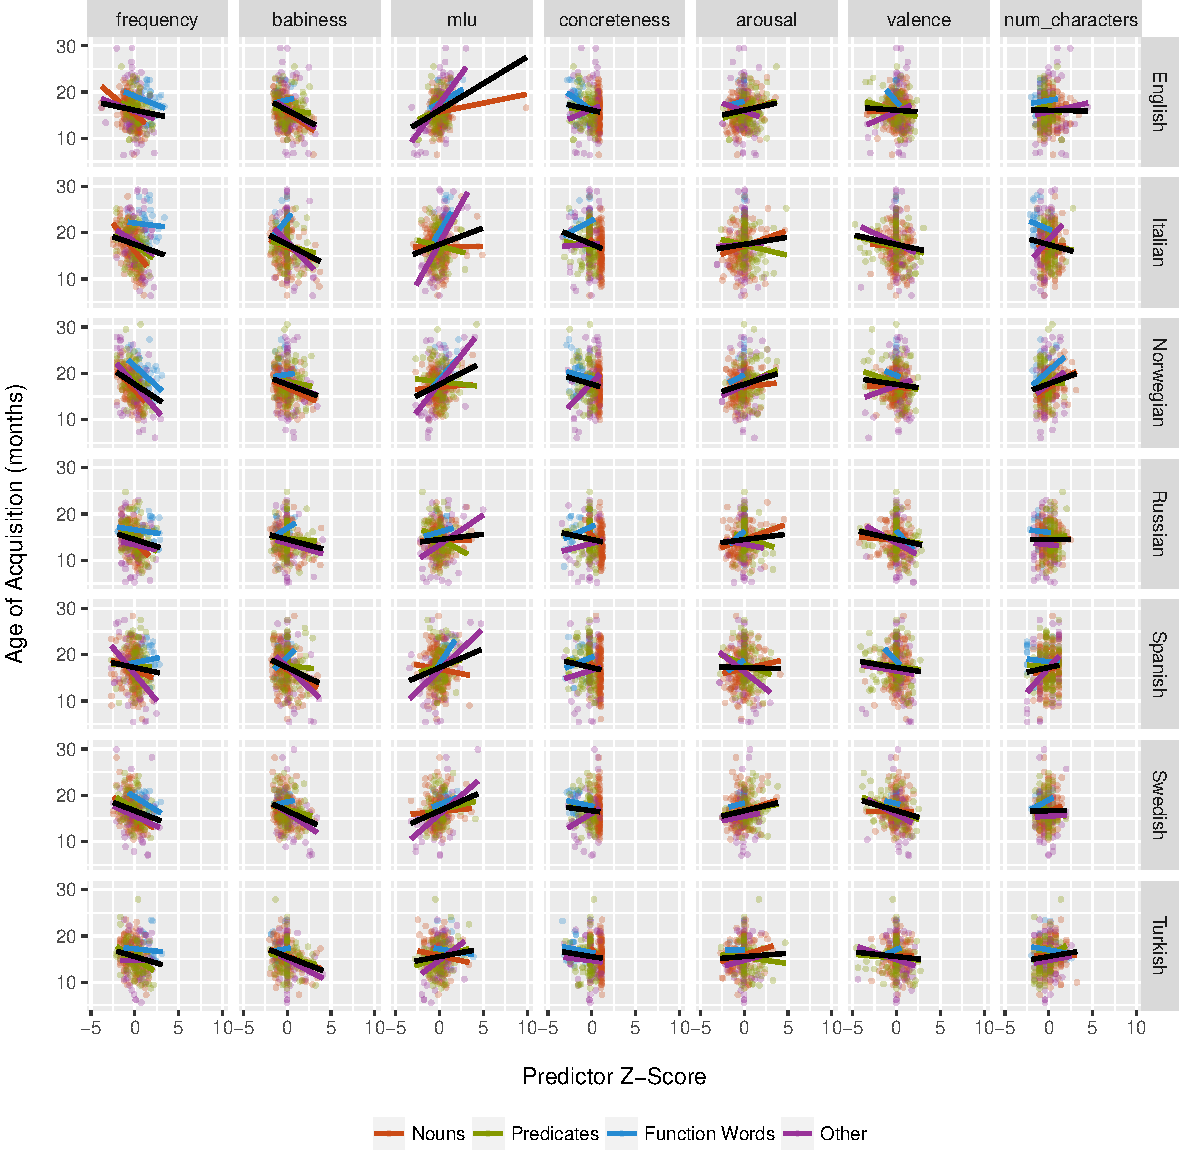
\includegraphics{aoapred_files/figure-latex/unnamed-chunk-2-1} 

}

\caption{Example production trajectories for the words "dog" and "jump" across languages. Points show average proportion of children producing each word for each one-month age group. Lines show the best-fitting logistic curve. Labels show the forms of the word in each language.}\label{fig:unnamed-chunk-2}
\end{figure*}

For each word, CDI data yield a trajectory reflecting the number of
children that are reported to produce or understand the word at each age
covered by the instrument (see Figure 1 for some examples). We then use
a mixed-effects logistic regression model to predict whether each child
knows the word on the basis of the child's age, properties of the word,
and interactions between age and each property of the word. We also fit
such models separately to the words in each lexical category. The
magnitude of the standardized coefficient on each feature gives an
estimate of its importance in predicting whether words are learned
earlier or later. Interactions between features and age give estimates
of how this effect is modulated for earlier and later-learned words. For
example, a positive effect of association with babies
(\enquote{babiness}) means that words associated with babies are learned
earlier; a negative interaction with age means that high babiness
primarily leads to higher rates of production and comprehension for
younger children.

\begin{table}[t]
\centering
\begin{tabular}{lll}
  \hline
Predictor & Highest & Lowest \\ 
  \hline
Babiness & baby, bib, bottle & donkey, penny, jeans \\ 
  MLU & when, day, store & peekaboo, ouch, hello \\ 
  Frequency & you, it, that & cockadoodledoo, grrr, church \\ 
  Concreteness & apple, baby, ball & how, now, that \\ 
  Solo frequency & no, yes, what & tooth, feed, aunt \\ 
  Arousal & naughty, money, scared & shh, asleep, blanket \\ 
  Length & cockadoodledoo, refrigerator, rocking chair & i, go, hi \\ 
  Valence & happy, hug, love & sick, hurt, ouch \\ 
  Final frequency & book, it, there & give, when, put \\ 
   \hline
\end{tabular}
\caption{Items with the highest and lowest values for each predictor in English.} 
\label{table:extremes}
\end{table}

\begin{figure*}

{\centering \includegraphics{aoapred_files/figure-latex/unnamed-chunk-3-1} 

}

\caption{Estimates of coefficients in predicting words' developmental trajectories. Each point represents a predictor's coefficient in one language, with the large point showing the mean across languages. Larger coefficient values indicate a greater effect of the predictor on acquisition: positive main effects indicate that words with higher values of the predictor tend to be understood/produced by more children, while negative main effects indicate that words with lower values of the predictor tend to be understood/produced by more children; positive age interactions indicate that the predictor's effect increases with age, while negative age interactions indicate the predictor's effect decreases with age.}\label{fig:unnamed-chunk-3}
\end{figure*}

Each of our predictors is derived from independent sources. For each
word that appears on the CDI forms in each of our 10 languages, we used
corpora of child-directed speech in that language to obtain an estimate
of its frequency, the mean length of utterances in which it appears, its
frequency as the sole consituent of utterance, and its frequency in
utterance final position (with frequency residualized out of solo and
final frequencies). Additionally, we computed each word's length in
characters and included ratings of its concreteness, valence, arousal,
and relatedness to babies. Since existing datasets for conceptual
ratings are primarily available for English, we mapped all words onto
translation equivalents across CDI forms, verified by native speaker
judgements, allowing us to use the ratings for English words across
languages. While necessarily imperfect, this method allows us to examine
languages for which limited resources exist. Example words for these
predictors in English are shown in Table 2.

A potential concern for comparing coefficient estimates is predictor
collinearity. Fortunately, in every language, the highest correlations
were between MLU and solo frequency (mean over languages and measures
\emph{r = } -0.50), as expected given the similarity of these factors;
and frequency and number of characters (mean over languages and measures
\emph{r = } -0.40), a reflection of Zipf's Law (32).

\section*{Results}\label{results}
\addcontentsline{toc}{section}{Results}

Figure 2 shows the coefficient estimate for each predictor in each
language. We find that babiness, frequency, MLU, and concreteness are
relatively stronger predictors of age of acquisition across languages.
Given the emphasis on frequency effects in the language acquisition
literature (33), one might have expected frequency to dominate, but
several other predictors are just as strong in this analysis. Some
factors previously argued to be important for word learning, namely
valence and arousal (34), appear to have limited relevance when compared
to other factors.

\begin{figure}

{\centering \includegraphics{aoapred_files/figure-latex/unnamed-chunk-4-1} 

}

\caption{Correlations of coefficients estimates between languages. Each point represents the mean of one language's coefficients' correlation with each other language's coefficients, with the black line indicating the overall mean across languages. The grey region and dashed line show a bootstrapped 95\% confidence interval of a randomized baseline where predictor coefficients are shuffled within language.}\label{fig:unnamed-chunk-4}
\end{figure}

\begin{figure*}

{\centering \includegraphics{aoapred_files/figure-latex/unnamed-chunk-5-1} 

}

\caption{Estimates of coefficients in predicting words' developmental trajectories (as described in Figure 2), with separate models for each lexical category.}\label{fig:unnamed-chunk-5}
\end{figure*}

Overall, there is considerable consistency in the magnitudes of
predictors across languages. In almost all, babiness and frequency were
highest, while valence and arousal were smaller. A priori it could have
been the case that different languages have wildly different effects of
experiential vs.~structural factors, but this pattern is not what we
observe. Instead, Figure 3 shows the mean pairwise correlation of
predictor coefficients across languages (i.e., the correlation of
coefficients for English with coefficients for Russian, for Spanish, and
so on). These means -- and even the individual datapoints -- are far
outside of bootstrapped estimates for the average pairwise correlation
in a randomized baseline created by shuffling predictor coefficients
within language, suggesting that coefficient estimates are far more
consistent across languages than would be expected by chance.

Word length is the one predictor of acquisition that varied
substantially between measures, in that it is far more predictive for
production than comprehension. Thus as measured here, length seems to be
playing more the role of production constraints (i.e., how difficult a
word is to say) than comprehension constraints (i.e., how difficult it
is to store or access).

Next, we wanted to examine how the relative contributions of the
predictors changes over development. Across languages, positive age
interactions can be seen for concreteness and frequency (i.e., their
effects increase with age). Conversely, there are negative age
interactions for babiness and valence in comprehension and for solo
frequency in production, suggesting stronger effects in words learned
earlier in development.

Previous work gives reason to believe that predictors' relationship with
age of acquisition differs among various lexical categories (7). To
investigate these effects, we separated our data by lexical category and
fit separate models for each category. Figure 4 shows the resulting
coefficient estimates. Across languages, frequency had the highest
magnitude for nouns and a lower magnitude for function words. In
contrast, MLU was almost irrelevant for both nouns and predicates, but
highly predictive for function words. These patterns are supportive of
the hypothesis that different word classes are learned in different
ways, or at least that the bottleneck on learning tends to be different,
leading to different information sources being more or less important
across categories.

\section*{Discussion}\label{discussion}
\addcontentsline{toc}{section}{Discussion}

What makes words easier or harder for young children to learn? Previous
experimental work has largely addressed this question using small-scale
experiments. While such experiments can identify sources of variation,
they typically do not allow for different sources to be compared in
detail. In contrast, observational studies allow the effects of
individual factors to be measured across ages and lexical categories (7,
8, 12). Such work has identified a number of candidate predictors of
word learning. By including 10 languages and 9 predictors, our work
expands the scope of these studies dramatically, leading to several new
findings.

First, we found general consistency in the ordering of predictors across
languages, at a level substantially greater than the predictions of a
chance model. This consistency supports the idea that differences in
culture or language structure do not lead to fundamentally different
acquisition strategies, at least at the level of detail we were able to
examine. Instead, they may be produced by \enquote{process universals}:
learning mechanisms and biases that are similar across children (at
least in the aggregate) and lead to the observed ordering of factors.
This account is highly speculative, however. Testing it further would
require both the addition of data from other languages and language
families, as well as eventual experiments measuring learning biases
across children from different language communities.

Second, predictors varied substantially in their weights across lexical
categories. Frequent, concrete nouns were learned earlier, consistent
with theories that emphasize the importance of early referential speech
(35). But for predicates, concreteness was somewhat less important. And
for function words, MLU was most predictive, perhaps because it is
easiest to decode the meanings of function words that are used in short
sentences (or because such words have meanings that are easiest to
decode). Overall these findings are consistent with some predictions of
both division of dominance theory, which highlights the role of
conceptual structure in noun acquisition (17), and syntactic
bootstrapping theory, which emphasizes linguistic structure over
conceptual complexity in the acquisition of lexical categories other
than nouns (19). More generally, our methods here provide a way forward
for testing the predictions of these theories across languages and at
the level of the entire lexicon rather than individual words.

In addition to these new insights, several findings emerge that confirm
and expand previous reports. Environmental frequency was an important
predictor of learning, with more frequently heard words learned earlier
(7, 12). Predictors also changed in relative importance across
development. For example, certain words whose meanings were more
strongly associated with babies appeared to be learned early for
children across the languages in our sample (2). Finally, word length
showed a disassociation between comprehension and production, suggesting
that challenges in production do not carry over to comprehension (at
least in parent-report data).

Despite its larger scope, our work shares a number of important
limitations with previous studies. First and foremost, our approach is
to predict one set of individuals with data about the experience of a
completely different set and ratings of concepts gathered from yet
others. In contrast to dense-data analyses (11), this approach
fundamentally limits the amount of variability we will be able to
capture. In addition, the granularity of the predictors that can be
extracted from corpus data and applied to every word is necessarily
quite coarse. Ideally, predictors could be targeted more specifically at
particular theoretical constructs of interest (for example, the patterns
of use for specific predicates). Finally, our data are observations
gleaned from parent report and are subject to both causal confounding
and confounding via biases in parent observation. Thus, our conclusions
will require further testing through converging evidence from both
laboratory experiments and direct observation.

In sum, by examining predictors of early word learning across languages,
we identified substantial cross-linguistic consistency in the factors
contributing to the ease or difficulty of learning individual words.
These findings testify to the importance of building open, shared
resources in the study of language learning -- without the efforts of
many research groups across many language communities, such studies
would be impossible. In addition, we hope that our work here provides a
baseline for the building of future predictive models that allow
theories of language learning to be tested at scale.

\newpage

\section{Materials and Methods}\label{materials-and-methods}

All code and data to reproduce our analyses are available at
\texttt{https://github.com/mikabr/aoa-prediction}.

\subsection{Predictor variables}\label{predictor-variables}

Each numeric predictor was centered and scaled so that all predictors
would have comparable units. For each predictor, missing values (CDI
items that were not in the relevant corpus or norms) were imputed from
the mean for their respective language and measure. Placeholder items,
such as \enquote{child's own name}, were excluded.

Translation equivalents are available in the Wordbank database using the
\texttt{wordbankr} package in \texttt{R} (15). Translation equivalents
were constructed by the authors and independently hand-checked by native
speakers.

\subsubsection{Frequency}\label{frequency}

For each language, we estimated word frequency from unigram counts based
on all corpora in CHILDES for that language. Each word's count includes
the counts of words that share the same stem (so that \enquote{dogs}
counts as \enquote{dog}) or are synonymous (so that \enquote{father}
counts as \enquote{daddy}). For polysemous word pairs (e.g.,
\enquote{orange} as in color or fruit), occurrences of the word in the
corpus were split uniformly between the senses on the CDI. Counts were
normalized to the length of each corpus, Laplace smoothed, and then log
transformed.

\subsubsection{Solo and Final
Frequencies}\label{solo-and-final-frequencies}

Using the same dataset as for frequency, we estimated the frequency with
which each of word occurs as the sole word in an utterance, and the
frequency with which it appears as the final word of an utterance (not
counting single-word utterances). As with frequency, solo and final
counts were normalized to the length of each corpus, Laplace smoothed,
and log transformed. Since both of these estimates are by necessity
highly correlated with frequency, we then residualized unigram frequency
out of both of them, so that values reflect an estimate of the effect of
solo/final frequency over and above frequency itself.

\subsubsection{MLU}\label{mlu}

For each language, we estimated each word's MLU by calculating the mean
length in words of the utterances in which that word appeared, for all
corpora in CHILDES for that language. For words that occurred fewer than
10 times, MLU estimates were not used (i.e.~treated as missing).

\subsubsection{Length}\label{length}

We computed the number of characters in each word in each language.
While imperfect, this metric of length is highly correlated with number
of phonemes and syllables (36).

\subsubsection{Concreteness}\label{concreteness}

We used previously collected norms for concreteness (37), which were
gathered by asking adult participants to rate how concrete the meaning
of each word is on a 5-point scale from abstract to concrete.

\subsubsection{Valence and Arousal}\label{valence-and-arousal}

We also used previously collected norms for valence and arousal (38),
for which adult participants were asked to rate words on a 1-9
happy-unhappy scale (valence) and 1-9 excited-calm scale (arousal).

\subsubsection{Babiness}\label{babiness}

Lastly, we used previously collected norms of \enquote{babiness}, a
measure of association with infancy (10) for which adult participants
were asked to judge a word's association with babies on a 1-10 scale.

\subsection{Lexical category}\label{lexical-category}

Category was determined on the basis of the conceptual categories
presented on the CDI form (e.g., \enquote{Animals}), such that the Nouns
category contains common nouns, Predicates contains verbs and
adjectives, Function Words contains closed-class words, and Other
contains the remaining items (39).

\subsection{Analysis}\label{analysis}

For all analyses, we used logistic mixed-effects regression models (fit
with \texttt{lme4\ 1.1-12} in \texttt{R}) to predict whether each child
understands/produces each word from age, the above predictors, and the
interactions of age with the predictors. Each model was fit to all data
from a particular language community and included a random intercept for
each word and a random slope of age for each word.

\newpage

\section{Acknowledgements}\label{acknowledgements}

Thank you to the labs and individuals who contributed data to Wordbank
and to NSF BCS \#1528526 for support.

\section{Author Contributions}\label{author-contributions}

M.B. and D.Y. conducted data processing and analysis, with supervision
from V.A.M. and M.C.F.; all authors contributed to writing the paper.

\section{Competing Interest
Statement}\label{competing-interest-statement}

The authors declare no conflict of interest.

\newpage

\section{References}\label{references}

\setlength{\parindent}{-0.5in} \setlength{\leftskip}{0.5in}

\hypertarget{refs}{}
\hypertarget{ref-fenson2007}{}
1. Fenson L, et al. (2007) \emph{MacArthur-Bates Communicative
Development Inventories} (Brookes Publishing Company).

\hypertarget{ref-tardif2008}{}
2. Tardif T, et al. (2008) Baby's first 10 words. \emph{Developmental
Psychology} 44(4):929.

\hypertarget{ref-schneider2015}{}
3. Schneider R, Yurovsky D, Frank MC (2015) Large-scale investigations
of variability in children's first words. \emph{Proceedings of the
Cognitive Science Society}.

\hypertarget{ref-mayor2014}{}
4. Mayor J, Plunkett K (2014) Shared understanding and idiosyncratic
expression in early vocabularies. \emph{Developmental science}
17(3):412--423.

\hypertarget{ref-fenson1994}{}
5. Fenson L, et al. (1994) Variability in early communicative
development. \emph{Monogr Soc Res Child Dev} 59(5).

\hypertarget{ref-mayor2011}{}
6. Mayor J, Plunkett K (2011) A statistical estimate of infant and
toddler vocabulary size from CDI analysis. \emph{Dev Sci}
14(4):769--785.

\hypertarget{ref-goodman2008}{}
7. Goodman JC, Dale PS, Li P (2008) Does frequency count? Parental input
and the acquisuisition of vocabulary. \emph{J Child Lang} 35(3):515.

\hypertarget{ref-hills2009}{}
8. Hills TT, Maouene M, Maouene J, Sheya A, Smith L (2009) Longitudinal
analysis of early semantic networks: Preferential attachment or
preferential acquisuisition? \emph{Psychol Sci} 20(6):729--739.

\hypertarget{ref-stokes2010}{}
9. Stokes SF (2010) Neighborhood density and word frequency predict
vocabulary size in toddlers. \emph{J Speech Lang Hear Res}
53(3):670--683.

\hypertarget{ref-perry2015}{}
10. Perry LK, Perlman M, Lupyan G (2015) Iconicity in English and
Spanish and its relation to lexical category and age of acquisuisition.
\emph{PloS One} 10(9):e0137147.

\hypertarget{ref-roy2015}{}
11. Roy BC, Frank MC, DeCamp P, Miller M, Roy D (2015) Predicting the
birth of a spoken word. \emph{Proc Natl Acad Sci} 112(41):12663--12668.

\hypertarget{ref-swingley2017}{}
12. Swingley D, Humphrey C (2017) Quantitative linguistic predictors of
infants' learning of specific English words. \emph{Chi Dev}.

\hypertarget{ref-slobin1985}{}
13. Slobin DI (1985) \emph{The crosslinguistic study of language
acquisition: Theoretical issues} (Psychology Press).

\hypertarget{ref-bates1987}{}
14. Bates E, MacWhinney B (1987) Competition, variation, and language
learning. \emph{Mech of Lang Acquis}:157--193.

\hypertarget{ref-frank2016}{}
15. Frank MC, Braginsky M, Yurovsky D, Marchman VA (2016) Wordbank: An
open repository for developmental vocabulary data. \emph{J Child Lang}.

\hypertarget{ref-macwhinney2000}{}
16. MacWhinney B (2000) \emph{The CHILDES project: The database}
(Psychology Press).

\hypertarget{ref-gentner2001}{}
17. Gentner D, Boroditsky L (2001) Individuation, relativity, and early
word learning. \emph{Lang Acquis and Concept Dev} (Cambridge University
Press).

\hypertarget{ref-gleitman1990}{}
18. Gleitman L (1990) The structural sources of verb meanings.
\emph{Lang Acquis} 1(1):3--55.

\hypertarget{ref-snedeker2007}{}
19. Snedeker J, Geren J, Shafto CL (2007) Starting over: International
adoption as a natural experiment in language development. \emph{Psychol
Sci} 18(1):79--87.

\hypertarget{ref-kovacevic1996}{}
20. Kovacevic M, Babic Z, Brozovic B (1996) A Croatian language parent
report study: Lexical and grammatical development. \emph{Seventh
International Congress for the Study of Child Language, Istanbul,
Turkey}.

\hypertarget{ref-bleses2008}{}
21. Bleses D, et al. (2008) The Danish Communicative Developmental
Inventories: Validity and main developmental trends. \emph{J Child Lang}
35(03):651--669.

\hypertarget{ref-boudreault2007}{}
22. Boudreault M, Cabirol E, Poulin-Dubois D, Sutton A, Trudeau N (2007)
MacArthur Communicative Development Inventories: Validity and
preliminary normative data. \emph{La Revue d'Orthophonie et
d'Audiologie} 31(1):27--37.

\hypertarget{ref-trudeau2011}{}
23. Trudeau N, Sutton A (2011) Expressive vocabulary and early grammar
of 16-to 30-month-old children acquisuiring Quebec French. \emph{First
Lang} 31(4):480--507.

\hypertarget{ref-caselli2012}{}
24. Caselli MC, Rinaldi P, Stefanini S, Volterra V (2012) Early action
and gesture ``vocabulary'' and its relation with word comprehension and
production. \emph{Chi Dev} 83(2):526--542.

\hypertarget{ref-caselli1995}{}
25. Caselli MC, et al. (1995) A cross-linguistic study of early lexical
development. \emph{Cog Dev} 10(2):159--199.

\hypertarget{ref-simonsen2014}{}
26. Simonsen HG, Kristoffersen KE, Bleses D, Wehberg S, Jørgensen RN
(2014) The Norwegian communicative development inventories: Reliability,
main developmental trends and gender differences. \emph{First Lang}
34(1):3--23.

\hypertarget{ref-vershinina2011}{}
27. Vershinina E, Yeliseyeva M (2011) Some norms of speech development
of children from 8 to 18 months. \emph{Special Education}.

\hypertarget{ref-yeliseyeva2009}{}
28. Yeliseyeva M, Vershinina E (2009) Some norms of speech development
of children from 18 to 36 months (based on the materials of the
MacArthur survey). \emph{Problems of Developmental Linguistics,
Saint-Petersburg}, p 22.

\hypertarget{ref-fenson2003}{}
29. Jackson-Maldonado D, et al. (2003) \emph{MacArthur Inventarios del
Desarrollo de Habilidades Comunicativas: User's guide and technical
manual} (Brookes Publishing Company).

\hypertarget{ref-eriksson2002}{}
30. Eriksson M, Berglund E (2002) \emph{Instruments, scoring manual and
percentile levels of the Swedish Early Communicative Development
Inventory, SECDI} (Högskolan i Gävle).

\hypertarget{ref-acarlar2008}{}
31. Acarlar F, et al. (2008) Adapting MB-CDI to Turkish: The first
phase. \emph{Essays of Turkish Linguistics: Proceedings of the 14th
International Conference on Turkish Linguistics}, pp 6--8.

\hypertarget{ref-zipf1935}{}
32. Zipf GK (1935) The psycho-biology of language.

\hypertarget{ref-ambridge2015}{}
33. Ambridge B, Kidd E, Rowland CF, Theakston AL (2015) The ubiquity of
frequency effects in first language acquisuisition. \emph{J Child Lang}
42(02):239--273.

\hypertarget{ref-moors2013}{}
34. Moors A, et al. (2013) Norms of valence, arousal, dominance, and age
of acquisuisition for 4,300 dutch words. \emph{Behav Res Meth}
45(1):169--177.

\hypertarget{ref-baldwin1995}{}
35. Baldwin DA (1995) Understanding the link between joint attention and
language. \emph{Joint Attention}:131--158.

\hypertarget{ref-lewis2016}{}
36. Lewis ML, Frank MC (2016) The length of words reflects their
conceptual complexity. \emph{Cognition} 153:182--195.

\hypertarget{ref-brysbaert2014}{}
37. Brysbaert M, Warriner AB, Kuperman V (2014) Concreteness ratings for
40 thousand generally known English word lemmas. \emph{Behav Res Meth}
46(3):904--911.

\hypertarget{ref-warriner2013}{}
38. Warriner AB, Kuperman V, Brysbaert M (2013) Norms of valence,
arousal, and dominance for 13,915 English lemmas. \emph{Behav Res Meth}
45(4):1191--1207.

\hypertarget{ref-bates1994}{}
39. Bates E, et al. (1994) Developmental and stylistic variation in the
composition of early vocabulary. \emph{J Child Lang} 21(01):85--123.






\end{document}
